\documentclass[tikz,convert={outfile=\jobname.svg}]{standalone}
%\usepackage{graphicx} % Required for inserting images
%\usepackage{tikz}
\usetikzlibrary{arrows, automata, positioning, fit, shapes.geometric, calc}
\begin{document}
%\centering

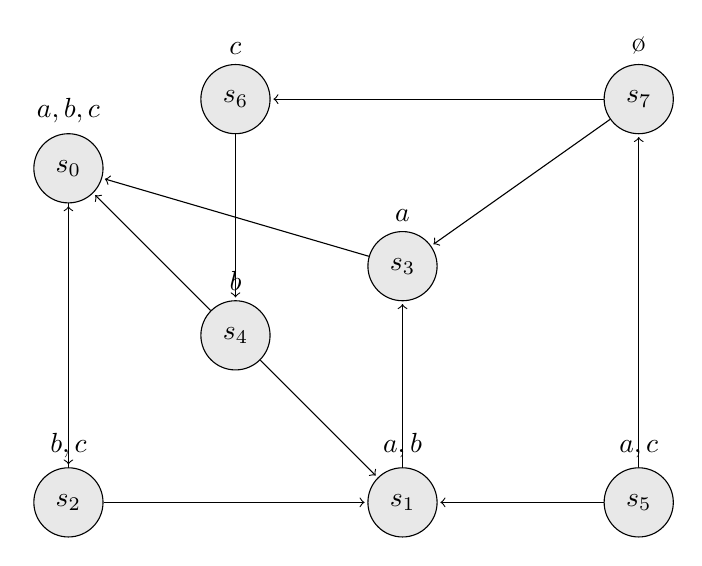
\begin{tikzpicture}[shorten >= 1pt, node distance=3cm, on grid, auto]
    \tikzstyle{every state}=[fill={rgb:black,1;white,10}]
    
    \node[state, label = {$a,b,c$}] (s_0) {$s_0$};
    \node[state] [below right of = s_0, label = {$b$}](s_4) {$s_4$};
    \node[state] [below left of = s_4, label = {$b,c$}](s_2) {$s_2$};
    
    \node[state] [below right of = s_4, label = {$a,b$}](s_1) {$s_1$};
    
    \node[state] [above of = s_1, label = {$a$}](s_3) {$s_3$};
    \node[state] [right of = s_1, label = {$a,c$}](s_5) {$s_5$};
    
    \node[state] [above of = s_4, label = {$c$}](s_6) {$s_6$};
    
    \node[state, label = \o] (s_7) at (s_6 -| s_5) {$s_7$};

    \path[->]
    (s_0) edge[] node{} (s_2)
    
    (s_1) edge[] node{} (s_3)

    (s_2) edge[] node{} (s_0)
          edge[] node{} (s_1)

    (s_3) edge[] node{} (s_0)
    
    (s_4) edge[] node{} (s_0)
          edge[] node{} (s_1)
    
    (s_5) edge[] node{} (s_1)
          edge[] node{} (s_7)
          
    (s_6) edge[] node{} (s_4)
          
    (s_7) edge[] node{} (s_3)
          edge[] node{} (s_6);
\end{tikzpicture}
\end{document}
